\documentclass[conference]{IEEEtran}
\IEEEoverridecommandlockouts
% The preceding line is only needed to identify funding in the first footnote. If that is unneeded, please comment it out.

% Custom packages
\usepackage{xspace}
\usepackage{hyperref}

% Custom useful commands
\newcommand{\criu}{\textsc{CRIU}\xspace}
\newcommand{\redis}{\textsc{Redis}\xspace}
\newcommand{\runc}{\texttt{runC}\xspace}

\usepackage{cite}
\usepackage{amsmath,amssymb,amsfonts}
\usepackage{algorithmic}
\usepackage{graphicx}
\usepackage{textcomp}
\usepackage{xcolor}
\def\BibTeX{{\rm B\kern-.05em{\sc i\kern-.025em b}\kern-.08em
    T\kern-.1667em\lower.7ex\hbox{E}\kern-.125emX}}
\begin{document}

\title{Live Migration of Container Networks with CRIU \\
\thanks{Identify applicable funding agency here. If none, delete this.}
}

\author{
    \IEEEauthorblockN{
        Carlos Segarra}
        \IEEEauthorblockA{
        \textit{Universitat Polit\`ecnica de Catalunya}\\
        Barcelona, Spain \\
        carlos.segarra@estudiant.upc.edu \\
        ORCID: 0000-0003-3455-7563
    }
\and
\IEEEauthorblockN{Jordi Guitart}
\IEEEauthorblockA{
    \textit{Computer Architecture Department} \\
    \textit{Universitat Polit\`ecnica de Catalunya}\\
    Barcelona, Spain \\
    jguitart@ac.upc.edu
}
}

\maketitle

\begin{abstract}
    One of the major hurdles for containers to become the cloud tenants' choice for application sandboxing is fault-tolerancy and load balancing.
    Checkpoint/Restore provides an efficient solution as it enables to save snapshots of running programs from which execution can be restored.
    Checkpointing and live migration for virtual machines has been around for several years now and, albeit less efficient, it provides with the robustness that a datacenter requires.
    However, checkpoint/restore (C/R) of running containers is still an open and active area of research.
    The biggest attempt to filling such a gap is Checkpoint-Restore in Userspace (CRIU) a software tool designed to dump, manage, and restore running processes by leveraging existing interfaces of the Linux Kernel.
    It does so completely from user-space and fully transparently.

    In this work we present a proof of concept implementation for live migration of established TCP connections of runC containers.
    Although C/R of established sockets is already available with \criu, migrating such a connection is left to the user, hence the novelty of our holistic approach.
    We also present a benchmark of the downtime experienced by a client when a network-intensive server is dumped and restored.
    Lastly, this short paper is a work in progress towards achieving C/R of container clusters to provide tools such as \textsc{Kubernetes} with fast restore times in the event of a node failure.
\end{abstract}


\begin{IEEEkeywords}
containers, checkpoint, restore, criu, runc
\end{IEEEkeywords}

\section{Introduction} \label{sec:introduction}

Containers have become the \textit{de-facto} alternative for managing application's lifecycle in the cloud.
With the progressive shift from bare-metal, to virtualized servers, and now with containerization, cloud tenants aim to find the balance between optimal resource usage and quality of service perceived by the user.
Microservices, serverless, cloud-native, are 


\section{Background Concepts} \label{sec:background}

This project builds on two foundational concepts of computer systems: containers, and checkpoint-restore.

\subsection{\criu: Checkpoint-Restore in Userspace}

Checkpoint/Restore in Userspace (\criu) is an open-source C/R tool~\cite{criu-main-page}.
Introduced in 2011, it's distinctive feature is that it is mainly implemented in user space, rather than in the kernel, by using existing interfaces~\cite{Reber2016}.
One of the most important interface is \texttt{ptrace}~\cite{ptrace-manpage}, as it relies on it for seizing the target process.
For other interfaces, several patches have been pushed to the mainline kernel by \criu developers~\cite{criu-kernel-patches}.
The project is currently under active development~\cite{criu-github}, and its main focus is to support the migration of containers.

\subsubsection{A Technical Overview on \criu}

The main goal of \criu is to perform a snapshot the current process' tree state to a set of image files, so that it can be later restored that exact point in time, without reproducing the steps that led to it.

\subsubsection*{Checkpoint}

The checkpointing process starts with the process identifier (PID) of a process group leader provided by the user through the command line using the \texttt{--tree} option~\cite{criu-checkpoint}.
However, before it can actually start, we need to ensure that the process does not change it's state during checkpoint.
This includes: opening file descriptors, changing sessions, or even producing new child processes~\cite{criu-freeze}.
To achieve this transparently, instead of sending a stop signal (which could affect the process' state) \criu freezes tasks using \texttt{ptrace}'s \texttt{PTRACE\_SEIZE} command~\cite{ptrace-manpage}.
In order to find all active tasks descendant of the parent PID, the \texttt{\$pid} dumper iterates through each \texttt{/proc/\$pid/task/} entry, recursively gathering threads and their children from \texttt{/proc/\$pid/task/\$tid/children}.

Once all tasks are frozen, \criu collects all the information it can about the task's resources.
File descriptors and registers are dumped through a \texttt{ptrace} interface and are parsed from \texttt{/proc/\$pid/fd} and \texttt{/proc/\$pid/stat} respectively.
In order to dump the contents of memory and credentials, a novel technique is introduced, the \textbf{parasite code}.

The parasite code is a binary blob built as a position independent executable (PIE) for execution inside another process adress space.
It's purpose is to execute \criu calls from within the dumpee's task address space~\cite{criu-parasite-code}.
To achieve this goal, \criu must:
\begin{enumerate}
    \item Move task into seized state calling \texttt{ptrace(PTRACE\_SEIZE, ...)}. Note that the task is stopped without it noticing, hence not altering it's state.
    \item Inject an \texttt{mmap} syscall in the current stack's instruction pointer, and allocate memory for the whole code blob. At this stage, space for exchanging parameters and results is also allocated within the dumpee's process adress space. \criu is now ready to run parasite service routines.
    \item The external dumping process retrieves information about the dumpee's adrress space through the parasite code either through \emph{trap} mode (one command at a time) or \texttt{daemon} mode (in which the parasite behavies as a UNIX socket.
    \item With information about used memory areas and important flags read from \texttt{/proc/\$pid/smaps/} and \texttt{/proc/\$pid/pagemap}, the parasite code transfers the actual content outside through a set of pipes, which in turn gets translated into image files.
\end{enumerate}
Lastly, the target process is cured from the parasite by closing it, unmapping it's allocated memory area, and reverting to the original frozen state.

\subsubsection*{Restore}

During the restore process, \criu morphs into the to-be-restored task.
Since we checkpoint process trees rather than single processes, \criu must \texttt{fork} itself several times to recreate the original PID tree.
In particular, and in order to be completely transparent, \criu requires that the restored tasks have the same PID they had before dump.
To achieve this goal, older versions of \criu had to perform very time-sensitive and race condition-prone PID handling, what was referred to as the PID dance~\cite{Reber2019,criu-pid-dance}.
Starting with kernel 5.3 and the new \texttt{clone3()} system call, it becomes now possible to clone a process and specify the desired PID for it~\cite{kernel-clone3}.

Then \criu restores all basic task resources such as file descriptors, namespaces, maps, ...
The only resources that are \emph{not} restored at this stage are, most notably, memory mappings.
In order to restore memory areas, and since the morphing is done \textit{in-place}, before exitting \criu would have to unmap itself and map the application code.
To overcome this issue, a similar approach to the parasite code one is followed, the \textbf{restorer blob}.
The restorer blob is a piece of PIE code, to which \criu transfers control to unmap itself and map the appropriate code and memory areas for the process to restore successfully.

\subsection{\runc: OCI-compliant container runtime}


\section{Checkpoint/Restore of Established Connections} \label{sec:system}

\subsection{Implementation in \criu}

\subsection{Live migration and integration with \runc}

\subsection{How to efficiently reuse IP addresses?}


\section{Evaluation} \label{sec:evaluation}

\begin{figure}[h!]
    \centering
    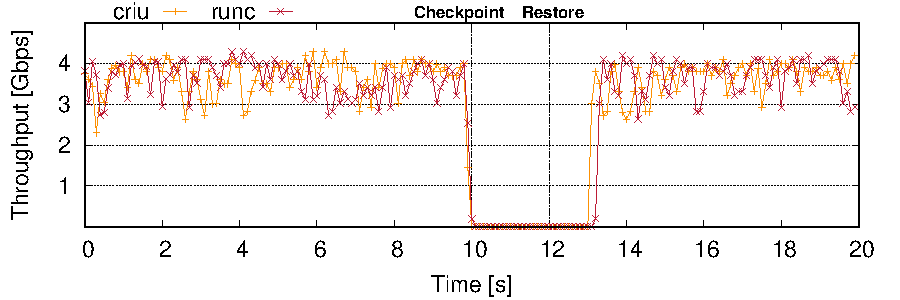
\includegraphics[width=\linewidth]{./images/tcp_established_downtime_microbenchmark.pdf}
    \caption{Throughput from the client as a function of time.\label{fig:evaluation-downtime}}
\end{figure}

\begin{figure}[h!]
    \centering
    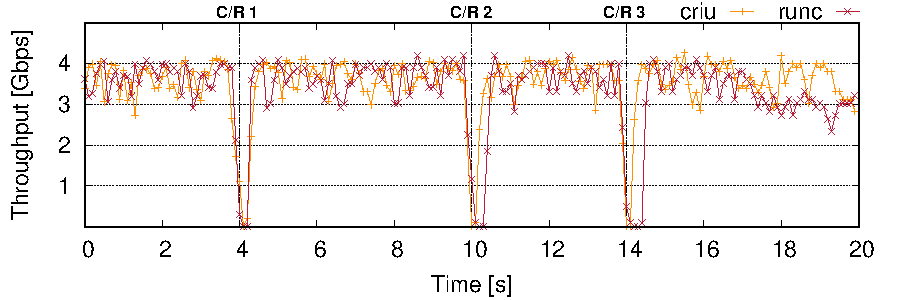
\includegraphics[width=\linewidth]{./images/tcp_established_resolution_microbenchmark.pdf}
    \caption{Throughput from the client as a function of time.\label{fig:evaluation-downtime}}
\end{figure}


\section{Related Work} \label{sec:related}


\section{Conclusions \& Future Work} \label{sec:conclusion}

In this short paper we have presented a preliminary evaluation of live migration of established TCP connections using Checkpoint-Restore In Userspace (CRIU).

In particular, we have implemented proofs of concept for migration between different machines and different namespaces within the same machine.
In addition to that, we have presented a benchmark of the impact of migrating a network-intensive server with regard to the perceived throughput from the client endpoint.
Our results show that migration introduces little overhead whereas checkpointing and restoring at a later point in time has an impact on connection restore time.
Lastly, our results also show that choosing to run the to-be-migrated server within a \runc container introduces minimal overhead when compared to checkpoint-restore of standalone processes.
As a consequence, we consider \criu to be mature enough to be integrated in bigger container stacks, particularly in container orchestrators were the ability to checkpoint established network connections could be of great use for load-balancing purposes.

Moving forward, we want to replicate the results here presented when migrating to different environments where migration speed could be the bottleneck, and the impact of traditional live migration techniques (such as pre-copy or lazy migration) could have to speed up the process.
We are also interested in evaluating the system on a more realistic use-case like an online gaming service, and integrate our work in an orchestrator tool to add support for distributed migration.


\bibliographystyle{unsrt}
\bibliography{biblio}

\end{document}
